\chapter{Why you should use GPG ?}

When I send emails or give my business card to people, I am continually
asked: What's GPG ? What is this file in your mail ?

\begin{figure}[htbp]
\centering
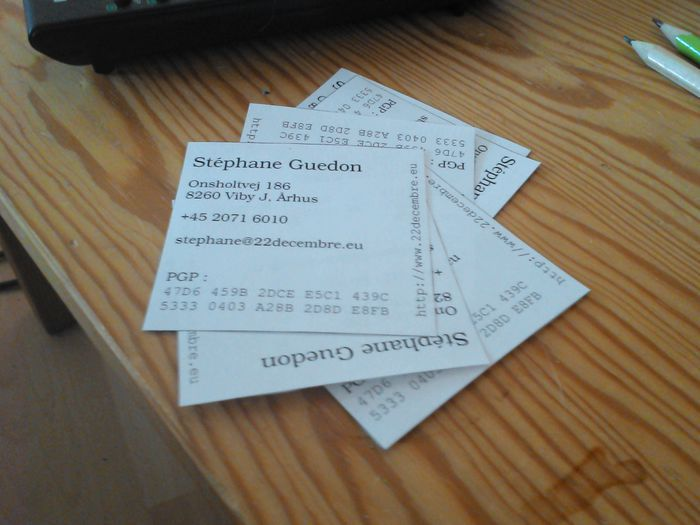
\includegraphics[width=0.7\linewidth]{./images/visiting.jpeg}
\caption{Business cards with a GPG key fingerprint}
\end{figure}

I am surprised that after Edward Snowden's disclosures about ongoing global surveillance\footnote{\url{http://en.wikipedia.org/wiki/Global_surveillance_disclosures_\%282013\%E2\%80\%93present\%29}} by secretive
American agencies (CIA, NSA\ldots{}), and the overwhelming power these secret agencies have, there are still many people - \emph{most poeple},
in fact ! - that don't know about GPG or personal privacy tools.

\section{What I am going to tell you}\label{what-i-am-going-to-tell-you}

Unlike the majority of tutorials over the web about GPG, I am going to
teach you on an incremental way, so it's easier for you to understand.

My purpose in doing this is to ensure that you know what you need to
know so that you're well-prepared by the time you need to use GPG in
practice. If you aren't well-prepared, it's easy to make a mistake that
renders the privacy GPG can offer you useless. So, we'll go one step at
a time to make sure you understand the whole thing and to allow yourself
to dive deeper at your own pace.

\section{What's GPG ?}\label{whats-gpg}

\subsection{In the beginning, there was PGP}\label{in-the-beginning-there-was-pgp}

PGP stands for \emph{Pretty Good Privacy}.

PGP is the original software, designed by Philip
Zimmermann\footnote{\url{http://philzimmermann.com/EN/background/index.html}}, whose goal was defending
privacy, individual liberties and more largely democracy\footnote{\url{http://www.philzimmermann.com/EN/essays/WhyIWrotePGP.html}}.

PGP is, first and foremost, a tool to encrypt, authenticate, and protect the contents of your email messages. This process uses a lot of
high-level math, but don't worry, because all of the math is done by the software itself.

\subsection{Then OpenPGP}\label{then-openpgp}

Then the IETF (Internet Engineering Task Force) standardized PGP format, leading to OpenPGP which made possible for every email user to exchange
encrypted emails with any other user, regardless of which email service, program, or provider they were actually using.

\subsection{Finaly came GPG}\label{finaly-came-gpg}

This allowed free-softwares advocates and developers to write a
software, GnuPG (the ``GNU Privacy Guard''), reduced to GPG, which implement OpenPGP. In other words :
with OpenPGP, GnuPG and PGP users can write and send mail to each other without any problem.

\section{Why would you want to use GPG ?}\label{why-would-you-want-to-use-gpg}

Are you in a couple ? Your partner send you hot pictures to make you horny, or you simply exchange hot talks you don't want anyone to read ?

You have a cooking competition and want to share your recipe for tarts with Bree Hodges, but not with Katherine Mayfair ?

You want to have your own business or are already working in a company and wish to discuss matters with your associates privately ?

You are a journalist and have to communicate with your sources in a safe way ? This case is very special, because ideally, your sources need to
feel confident that they can write to you in a way no one else can overhear even before they know you. It is important to notice that this
was Edward Snowden's case : he used PGP and asked his contacts to do the same to insure safe exchanges.

Some of these reasons seem shallow. But if we have learned one thing from \emph{Desperate Housewives} and people surrounding us, it's that no
matter how shallow or stupid it may seem, someone might want to open your mail and will use any measures they can to do it !\\
\\
But let's switch to something else. Ooooohhhh yeeesss\ldots{}\\
\\
Google\footnote{\url{http://www.huffingtonpost.com/2014/04/15/gmail-ads_n_5149032.html}}, Yahoo\footnote{\url{http://motherboard.vice.com/read/looking-up-symptoms-online-these-companies-are-collecting-your-data}} 
and Microsoft\footnote{\url{http://www.techworm.net/2014/10/microsofts-windows-10-permission-watch-every-move.html}} (Live and Hotmail for example) all read your email to create a profile about you, a dossier used to target advertisements, and worse.

Do you remember the fappening\footnote{\url{http://www.theguardian.com/world/2014/sep/01/nude-photos-of-jennifer-lawrence-and-others-posted-online-by-alleged-hacker}} ? The celebrities whose private, revealing photos have been stolen. Do you feel their reaction sane ? If so, why don't you value your own privacy the same ?\\
\\
Good news eventhough, apparently GPG is still safe\footnote{\url{http://www.ginjfo.com/actualites/politique-et-economie/espionnage-nsa-depose-les-armes-devant-certaines-solutions-cryptage-20141230}} !\\
\\
The thing you have to realize is that digital mail is not like sending a letter. It's more like sending a postcard. Anyone who looks can read
the contents. They don't have to open a sealed envelope to do it. So you can think of GPG as the envelope inside of which you put the
contents of your message. No more easy to read, intercept, or hijack postcards!

\section{But, Doctor, is it painful ?}\label{but-doctor-is-it-painful}

Let's say that encryption is not the easiest task on Earth. But I see no way or reason not to use it !

This is the reason I wrote this serie of articles, that you are now reading as a little book; to familiarize you with GPG so that you, too, will see no reason not to use it. By providing you a permanent documentation, by teaching you, gradually, to discover OpenPGP, I hope to allow you to protect your privacy and the
privacy of person's you love. You will see that after some training, using these tools is actually pretty easy and you do it in a natural way.